\documentclass[11pt,letterpaper]{article}
\usepackage[T1]{fontenc}
\usepackage[utf8]{inputenc}
\usepackage[margin=.94in,headheight=15pt]{geometry}
\usepackage{amsmath,amsthm,mathtools,newtxtext,newtxmath}
\usepackage{microtype,booktabs,array,tabularx,longtable,enumitem}
\usepackage{xcolor,tikz,fancyhdr,titlesec,needspace,placeins}
\usepackage{algorithm,algpseudocode,fontawesome5,xurl,hyperref}
\usetikzlibrary{arrows.meta,positioning,calc,fit}
\definecolor{ink}{HTML}{302045}
\definecolor{accent}{HTML}{6344A0}
\definecolor{muted}{HTML}{665E70}
\definecolor{gold}{HTML}{AC792C}
\definecolor{pale}{HTML}{F3F0F8}
\hypersetup{colorlinks=true,linkcolor=ink,citecolor=ink,urlcolor=accent,
 pdftitle={Autonomous Enterprises: Build the Means of Building},pdfauthor={Vincent Boucher},
 pdfsubject={Capability-producing computation and exact capital requirements for succession}}
\urlstyle{same}
\pagestyle{fancy}\fancyhf{}
\fancyhead[L]{\small\textsc{Autonomous Enterprises}}
\fancyhead[R]{\small Boucher / MONTREAL.AI}
\fancyfoot[C]{\thepage}\renewcommand{\headrulewidth}{.3pt}
\setlength{\parindent}{1.1em}\setlength{\parskip}{.15em}
\setlength{\emergencystretch}{2em}\renewcommand{\arraystretch}{1.12}
\setlist{nosep,leftmargin=1.5em,topsep=.3em}
\titleformat{\section}{\large\bfseries\color{ink}}{\thesection}{.6em}{}
\titleformat{\subsection}{\normalsize\bfseries}{\thesubsection}{.6em}{}
\titlespacing*{\section}{0pt}{1.2em}{.5em}
\titlespacing*{\subsection}{0pt}{.8em}{.3em}
\newcolumntype{Y}{>{\raggedright\arraybackslash}X}
\newcolumntype{P}[1]{>{\raggedright\arraybackslash}p{#1}}
\newcommand{\RR}{\mathbb R}\newcommand{\QQ}{\mathbb Q}\newcommand{\NN}{\mathbb N}
\newcommand{\M}{\mathcal M}\newcommand{\A}{\mathcal A}\newcommand{\B}{\mathcal B}
\newcommand{\Om}{SUCCESSOR~$\Omega$}
\newcommand{\thesis}[1]{\begin{center}\setlength{\fboxsep}{9pt}\fcolorbox{accent}{pale}{\begin{minipage}{.92\linewidth}#1\end{minipage}}\end{center}}
\DeclareMathOperator{\diag}{diag}\DeclareMathOperator{\pop}{popcount}
\newtheorem{theorem}{Theorem}[section]
\newtheorem{proposition}[theorem]{Proposition}
\newtheorem{corollary}[theorem]{Corollary}
\newtheorem{lemma}[theorem]{Lemma}
\theoremstyle{definition}\newtheorem{definition}[theorem]{Definition}
\theoremstyle{remark}\newtheorem{remark}[theorem]{Remark}
\renewcommand{\topfraction}{.95}\renewcommand{\bottomfraction}{.85}
\renewcommand{\textfraction}{.06}\renewcommand{\floatpagefraction}{.8}
\pdfinfoomitdate=1\pdftrailerid{}
\begin{document}
\thispagestyle{plain}
\begin{center}
{\small\sffamily\color{accent} MONTREAL.AI\quad /\quad TRANSFORMATIONAL INTELLIGENCE $\infty$}\par
\vspace{.7em}
{\Large\color{accent}\faStar\quad\faCogs}\par
\vspace{.6em}
{\fontsize{32}{36}\selectfont\bfseries\color{ink} Autonomous Enterprises\par}
\vspace{.5em}
{\Large\bfseries Build the Means of Building\par}
\vspace{.45em}
{\large Capability-Producing Computation and Exact Capital Requirements\par}
{\large for Succession\par}
\vspace{.8em}
{\large Vincent Boucher\par}
MONTREAL.AI\par
Montr\'eal, Qu\'ebec, Canada\par
\vspace{.4em}
21 October 2026\quad$\cdot$\quad Revised research manuscript
\end{center}
\begin{abstract}
An enterprise can finish with more cash and fewer affordable futures. A productive alternative may retain a tool that makes its successor cheaper to construct, even when a cash-only comparison would discard it. We make that difference executable. A capability-producing programme constructs a checked transform, uses it to construct a convolution operator, and uses the retained operators to reduce the work required to qualify an inverse solver. The successor's construction cost is measured within an explicit arithmetic work model rather than supplied as an unexplained fee. The mathematical contribution is an exact capital--capability retention law. For reserve-closed producer policies with different output stocks, it gives the worst additional launch capital caused by deleting alternatives, over every constructible capability target and nonnegative terminal cash target. A reconstruction path supplies the comparison; a critical successor supplies an attaining witness. The law requires operational concatenability, expressed by a directed triangle inequality, rather than submodular acquisition prices. We prove that this is its exact universal boundary over finite reflexive completion maps. In the executed foundry, inherited convolution reduces one inverse construction and qualification from 78,016 to 30,912 declared work units. Joint construction of three products costs 808,420 units, versus 1,226,276 for specified isolated builds; unrestricted joint planning matches the result. A separate exact example makes cash-only pruning raise successor launch capital from five to thirteen. Fresh checks cover 72 construction catalogues, 32,256 completion values and 28,472 capital targets. The previous edition's computations are reproduced. The result is a bounded mechanism for making productive inheritance and its financing jointly inspectable, not a new Fourier algorithm, an autonomous discovery of primitive laws, physical deployment or realized commercial growth.
\end{abstract}
\noindent\textbf{Keywords:} autonomous enterprises; transformational intelligence; capability production; certifying computation; constructive inheritance; capital requirements; SUCCESSOR $\Omega$.
\begin{center}\small
\textbf{Find your Alpha. Build your SUCCESSOR $\Omega$.}\par
\href{https://github.com/MontrealAI/AGI-Alpha-Agent-v0}{github.com/MontrealAI/AGI-Alpha-Agent-v0}
\end{center}
\clearpage

\section{The next product can be a better way to produce the next product}
Two enterprises complete the same current obligation. One takes the route that needs less starting money and returns more cash. The other retains a qualified computational factory. Judged only by those cash numbers, the factory route is dominated. Judged by what the next mission can actually construct, it may be indispensable.

This is not an accounting claim that a useful artifact can be spent like money. The artifact must do something. In our executed construction, a generated transform becomes an input to a new convolution programme. That checked programme then becomes part of the process used to qualify an inverse solver. Retaining it reduces the counted construction and checking work for that solver from 78,016 to 30,912 units. The new capability changes how another capability can be built.

\thesis{\textbf{Do not merely make the enterprise's next answer cheaper. Make its next capability cheaper to construct.}\par\smallskip
The durable output is not just a result or a surplus. It is a verified means of production, together with the resources, rights and evidence needed to use it.}

The previous edition of \emph{Autonomous Enterprises} established exact capital requirements for retaining policies of the \emph{same} capability type, and connected a checked measurement product to a modeled successor purchase \cite{previous}. That is useful, but it leaves two important restrictions. The next construction's cost was supplied, and the capital theorem could not compare plans that retained different productive assets. A cash-rich output-only route and a cash-poorer factory route have different successor possibilities. Giving them the same type erases the strategic question.

This revision removes those restrictions in a bounded setting. It constructs the productive dependency, records the work of creating and checking it, and proves a retention law that includes the cost of reconstructing missing capabilities. The paper's two principal results are therefore connected: the foundry makes reconstruction costs operational; the theorem says what losing that productive inheritance can cost the next mission.

\subsection{A concrete difference before the formalism}
The numerical foundry produces three different interfaces: linear interaction analysis, bilinear composition of independent binary effects, and inversion of a specified mixing operator. Their mathematics is classical. What the experiment tests is the construction history, the dependency on accepted predecessor artifacts, and the cost of checking a new product with or without that inheritance.

\begin{table}[htbp]\centering\small
\caption{The new executed comparison. Units are counted operations in the declared construction/checking model, not currency, wall-clock time or complete research cost.}
\begin{tabularx}{\linewidth}{@{}Yrr@{}}\toprule
Construction obligation & Without the named inheritance & With it\\\midrule
Construct and qualify one inverse, given the transform & 78,016 & 30,912\\
Construct all three products under the stated build architectures & 1,226,276 & 808,420\\\bottomrule
\end{tabularx}
\label{tab:opening}
\end{table}

The first saving is not merely skipping tests: both paths check every basis vector of the same operator identity. The inherited path executes a previously qualified convolution programme in the reference side of that identity. The second comparison charges the initial factory and failed construction candidates. It is an ablation of isolated versus shared construction, not a benchmark victory over an unrestricted compiler. A competent joint planner chooses the same sequence.

The economic difference is also exact. A supplied two-plan example has cash profiles $(2,8)$ and $(5,4)$, where the coordinates are required launch capital and net cash change. The first looks unconditionally better. The second leaves a factory that would cost twelve to reconstruct. For a named successor requirement, retaining the second plan reduces launch capital from thirteen to five. The apparent cash dominance was not productive dominance.

\subsection{What changes, and what does not}
The object of invention is a production arrangement: which computation, checker and financing path should remain after the present job so that a later job can construct a different capability. The accepted outputs are not weakened. The compiler may reorganize their realization; it may not remove the required mathematics, ignore qualification or convert an invented customer into funding.

Automatic transform generation, compositional verification, shortest-path planning and peak-resource accounting have substantial prior art \cite{spiral,certifying,dijkstra,kahn}. We use them directly. The new claims are the capital--capability identity, its exact compositional boundary, and a completed construction-and-inheritance study linked to that identity. No new Walsh transform or general autonomous-company superiority is claimed.

\section{One architecture, one foundation, six stages}
\label{sec:hierarchy}
\textbf{AGI ALPHA organizes intelligence.} Agents, tools, memory and validation form an accountable substrate. \textbf{Transformational intelligence changes the game.} It separates the authorized purpose from inherited ways of pursuing it and permits a better formulation only when the purpose is preserved \cite{ti}. The six stages produce the evidence and artifacts that \Om{} can inherit.

\begin{figure}[htbp]\centering
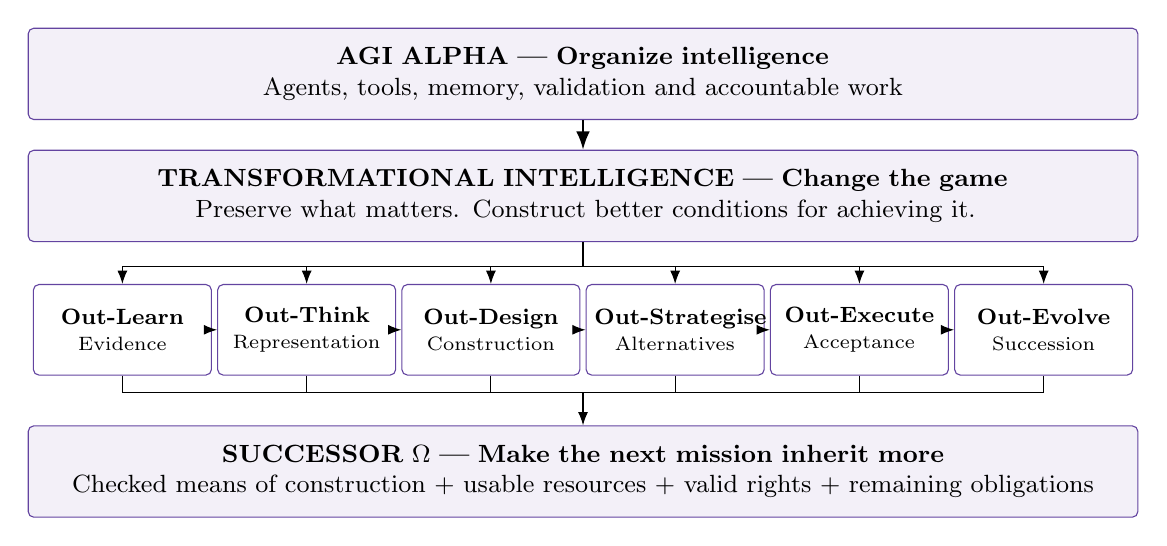
\begin{tikzpicture}[>=Latex,font=\small,
 box/.style={draw=accent,rounded corners=2pt,align=center,inner sep=7pt}]
\node[box,fill=pale,text width=13.6cm] (a) at (0,0) {\textbf{AGI ALPHA --- Organize intelligence}\par Agents, tools, memory, validation and accountable work};
\node[box,fill=pale,text width=13.6cm] (t) at (0,-1.55) {\textbf{TRANSFORMATIONAL INTELLIGENCE --- Change the game}\par Preserve what matters. Construct better conditions for achieving it.};
\draw[->,thick] (a)--(t);
\foreach \id/\x/\title/\sub in {1/-5.85/Out-Learn/Evidence,2/-3.51/Out-Think/Representation,3/-1.17/Out-Design/Construction,4/1.17/Out-Strategise/Alternatives,5/3.51/Out-Execute/Acceptance,6/5.85/Out-Evolve/Succession}{
 \node[box,text width=2.05cm,inner sep=3pt,minimum height=1.15cm,font=\footnotesize] (stage\id) at (\x,-3.25) {\textbf{\mbox{\title}}\par\scriptsize\sub};}
\foreach \a/\b in {1/2,2/3,3/4,4/5,5/6}{\draw[->] (stage\a.east)--(stage\b.west);}
\draw[-] (t.south)--(0,-2.45);
\draw[-] (-5.85,-2.45)--(5.85,-2.45);
\foreach \id in {1,2,3,4,5,6}{\draw[->] (stage\id.north |- 0,-2.45)--(stage\id.north);}
\node[box,fill=pale,text width=13.6cm] (s) at (0,-5.05) {\textbf{SUCCESSOR $\Omega$ --- Make the next mission inherit more}\par Checked means of construction + usable resources + valid rights + remaining obligations};
\draw[-] (stage1.south)--(-5.85,-4.05)--(5.85,-4.05)--(stage6.south);
\foreach \id in {2,3,4,5}{\draw[-] (stage\id.south)--(stage\id.south |- 0,-4.05);}
\draw[->] (0,-4.05)--(s.north);
\end{tikzpicture}
\caption{The organizing hierarchy. The six stages are logical responsibilities with feedback, not six compulsory agents or six measured levels of general intelligence. The new reference implements a bounded construction, planning and checking path within this architecture.}
\label{fig:hierarchy}
\end{figure}

The logical sequence is \textbf{Out-Learn $\to$ Out-Think $\to$ Out-Design $\to$ Out-Strategise $\to$ Out-Execute $\to$ Out-Evolve}. Learning determines which evidence and assumptions are justified. Thinking chooses a representation that preserves the relevant consequences. Design constructs a realization. Strategy keeps alternatives whose usefulness depends on future inheritance. Execution obtains and checks the actual result. Evolution changes what the next construction can use. These roles build on the supplied research sequence without combining incompatible mathematical assumptions \cite{learn,think,design,strategise,execute,evolve}.

In this paper, the representation is a typed capability stock and an operational construction graph. Design produces executable arithmetic programmes. Strategy compares policies that leave different stocks. Execution checks complete-domain identities in the admitted grammar. Succession uses those artifacts in another construction. The framework does not claim that its deterministic generator learned a better invention policy or that every named stage ran as an independent model agent.

\thesis{\textbf{A result becomes a verified capability. A capability becomes a means of constructing another capability.}\par\smallskip
The claim that capability compounds must identify the retained component, execute the new construction, preserve the old costs, and demonstrate the change in what can be built.}

\section{A capability is a construction that can be used, not an asset label}
\subsection{Qualified stocks and explicit recipes}
Let $\M$ be a finite catalogue of capability types. A valid stock $K\subseteq\M$ contains executable artifacts, checked contracts, compatible rights and the evidence required for their use. The types are optional and durable within the comparison: an unused tool causes no compulsory side effect, a digital routine is not consumed by invocation, and retaining more does not disable an admitted recipe. No physical capacity or permission is duplicated by copying a label.

A construction recipe $r$ specifies required capabilities $R_r$, produced capabilities $P_r$ and a deterministic nonnegative charge $c_r$. It is available when $R_r\subseteq K$ and changes the stock to $K\cup P_r$. Its charge includes the construction and checking operations declared by its resource model. A no-effect operation can be omitted. A zero-cost installation remains a real state change; a missing zero-priced component is not already present.

This is a deliberately finite construction language. In the foundry, a recipe invokes a bounded programme search, emits a structured artifact and performs a checker. In the generated tests, recipes are supplied contract tables. Neither a name nor a self-issued assertion establishes the physical truth of a contract. A new primitive, revised rights or changed operating condition creates a new qualification obligation.

\begin{definition}[Constructive completion cost]
For a qualified stock $K$ and target $Q$, let
\begin{equation}
 \rho(K,Q)=\min\left\{\sum_{r\in w}c_r:\ w\text{ is executable from }K,\ Q\subseteq K_w\right\}.
 \label{eq:rho}
\end{equation}
An unavailable target has cost $+\infty$. A finite minimum carries the actual recipe sequence and intermediate stock records, not only a scalar estimate.
\end{definition}

Costs may be money if independently priced in a common numeraire, or a specified computational resource. The two interpretations must not be mixed. Section~\ref{sec:work} counts work. Section~\ref{sec:finance} explicitly states the hypothetical tariff needed to translate that work into a funding example.

\subsection{Why construction changes the geometry of inheritance}
\begin{proposition}[Executable completion and concatenability]
\label{prop:completion}
For the finite optional-capability model, $\rho(K,K)=0$, and
\begin{align}
 K\subseteq L&\implies\rho(L,Q)\le\rho(K,Q),\label{eq:optional}\\
 \rho(L,Q)&\le\rho(L,K)+\rho(K,Q).\label{eq:triangle}
\end{align}
Exact search over installed subsets computes $\rho$ and a realizing path. A minimum path need contain at most $|\M\setminus K|$ stock-changing steps, although there can be exponentially many candidate stocks.
\end{proposition}
\begin{proof}
Doing nothing supplies reflexivity. Every recipe legal from $K$ remains legal from a superset, proving \eqref{eq:optional}. Execute a minimum path from $L$ to a stock containing $K$. From that stock, the path available from $K$ to $Q$ is still legal, with no larger charge. This proves \eqref{eq:triangle}, including extended-valued unavailable cases. Remove steps that produce no new capability. Every remaining step strictly enlarges the stock, even at zero cost, so there are at most $|\M\setminus K|$ of them. A shortest-path search over the finite stock graph gives the minimum and witness. A computational cap is incomplete search, not an impossibility proof.
\end{proof}

The triangle is an operational statement: one can first reconstruct the predecessor's means and then use them to build the requested successor. It does not say that the route through that predecessor is always best. A direct construction can be cheaper. The function is asymmetric, and distinct stocks can have zero completion cost; it is not an ordinary metric or a market valuation.

The reference implements nonnegative shortest paths \cite{dijkstra}. An independent target-specific dynamic programme visits states in decreasing stock size. It agrees on every saved construction value. The search method is standard; its task is to turn the enterprise's retained capabilities into inspectable future construction consequences.

\subsection{No submodular price assumption is necessary}
The earlier acquisition portfolio result used monotone submodular set prices \cite{strategise}. Here the cost is generated by executable routes, so it need not have that form. For example, buying any singleton $a,b,c$ costs two; constructing either package $\{a,b\}$ or $\{b,c\}$ also costs two. Then the from-scratch function $C(Q)=\rho(\varnothing,Q)$ has
\begin{equation}
 C(ab)+C(bc)=4 < C(b)+C(abc)=6.
 \label{eq:nonsubmod}
\end{equation}
It violates submodularity. Nevertheless, all reconstruction paths concatenate and \eqref{eq:triangle} holds. The exact continuation theorem below therefore applies. The improvement is not a claim that arbitrary cost tables are safe; it replaces a price-structure assumption with a constructive condition that can be checked.

\section{The exact capital cost of losing a productive inheritance}
\subsection{Bind cash and capability to the same completed policy}
A producer policy $p$ has summary
\begin{equation}
 p=(\kappa_p,\delta_p,K_p),\qquad \kappa_p\ge0,\quad\kappa_p+\delta_p\ge0.
 \label{eq:producer}
\end{equation}
Here $\kappa_p$ is the least opening capital that funds all represented prefixes, including reserves; $\delta_p$ is its least terminal free-cash change; $K_p$ is its qualified output stock. Both financial coordinates belong to the same realized contingent policy. All summarized terminal branches have the same usable stock and compatible boundary. Residual warranties, capacity, duration, ownership or permissions that differ across branches need a richer type, not silent averaging.

The previous paper derives these profiles from cash movements and reserve obligations and proves their finite-game synthesis \cite{previous}. Peak/net resource accounting itself is established \cite{kahn}. We preserve and reproduce that implementation rather than rename it. The extension here is that different producer alternatives may leave different $K_p$.

After producer completion, reconstruction uses the recipes of Section~3. Its charges are nonnegative, paid before the requested terminal boundary, and involve no intermediate sales receipts or new loans. They use the same accounting unit as the capital profile. Starting cash does not alter the stated construction tariffs or permissions. More general repair policies with their own receipts and credit constraints need the previous paper's full path interface; the scalar $\rho$ alone is insufficient.

\begin{proposition}[Capital required for a capability target]
\label{prop:capital}
To run $p$, then construct $Q$, and retain at least $x\ge0$ free cash, the least opening capital is
\begin{equation}
 H_p(Q,x)=\max\{\kappa_p,\ x-\delta_p+\rho(K_p,Q)\}.
 \label{eq:H}
\end{equation}
\end{proposition}
\begin{proof}
The producer must be funded, so the opening amount $b$ is at least $\kappa_p$. Its worst terminal free cash is $b+\delta_p$. Pure-expense reconstruction costs $\rho(K_p,Q)$, with no prefix more expensive than its nonnegative total; retaining $x$ therefore requires $b+\delta_p\ge \rho(K_p,Q)+x$. These conditions are necessary and are sufficient using an attaining construction path.
\end{proof}

For a finite nonempty portfolio $\A$ set
\begin{equation}
 F_\A(Q,x)=\min_{a\in\A}H_a(Q,x).
 \label{eq:portfolio}
\end{equation}
This minimum chooses a complete producer, not the seed of one and the factory of another. Once the successor target is known, a different whole producer may be optimal. The following guarantee covers every target without forecasting which will arrive.

\begin{theorem}[Exact capital--capability retention law]
\label{thm:main}
Let $\rho$ be finite, nonnegative and reflexive on the declared stock domain, and satisfy \eqref{eq:triangle}. Let $\A$ be a finite nonempty family of producers and $\varnothing\ne\B\subseteq\A$ a retained family. Then
\begin{equation}
 \boxed{\quad
 \sup_{Q,\,x\ge0}\big[F_\B(Q,x)-F_\A(Q,x)\big]
 =\max_{a\in\A}\min_{b\in\B}
 \max\{\kappa_b-\kappa_a,\ \delta_a-\delta_b+\rho(K_b,K_a)\}.
 \quad}
 \label{eq:main}
\end{equation}
A maximizing full producer $a_*$ supplies an attaining successor:
\begin{equation}
 Q_*=K_{a_*},\qquad x_*=\kappa_{a_*}+\delta_{a_*}.
 \label{eq:witness}
\end{equation}
Thus the exact largest extra launch requirement is certified by producer pairs and one reconstruction task per pair, rather than enumerating every future cash target and capability request.
\end{theorem}
\begin{proof}
For fixed $a,b$, put
\begin{equation}
 d(a,b)=\max\{\kappa_b-\kappa_a,\ \delta_a-\delta_b+\rho(K_b,K_a)\}.
 \label{eq:distance}
\end{equation}
The first coordinate gives $\kappa_b\le\kappa_a+d(a,b)$. The triangle gives
\begin{align}
 x-\delta_b+\rho(K_b,Q)
 &\le x-\delta_b+\rho(K_b,K_a)+\rho(K_a,Q)\notag\\
 &\le x-\delta_a+\rho(K_a,Q)+d(a,b).
 \label{eq:upper}
\end{align}
Taking the two maxima proves $H_b(Q,x)\le H_a(Q,x)+d(a,b)$. For an optimal full producer at $(Q,x)$, use its minimum-distance retained replacement. If $\Delta$ denotes the right-hand side of \eqref{eq:main}, this proves $F_\B\le F_\A+\Delta$.

Choose a maximizing $a_*$. At \eqref{eq:witness}, reflexivity gives $H_{a_*}=\kappa_{a_*}$ and hence $F_\A\le\kappa_{a_*}$. For every retained $b$,
\begin{equation}
 H_b(K_{a_*},x_*)-\kappa_{a_*}
 =\max\{\kappa_b-\kappa_{a_*},\delta_{a_*}-\delta_b+\rho(K_b,K_{a_*})\}.
\end{equation}
Minimizing over $b$ yields $F_\B-F_\A\ge\Delta$. The upper bound proves equality and attainment. Subportfolio inclusion makes the total loss nonnegative even though an individual $d(a,b)$ can be negative.
\end{proof}

The theorem measures \emph{additional required launch capital}, not the sale value of a factory. Its witness is a legitimate continuation question: reconstruct the full producer's output and preserve the cash available at its own minimum launch. It is not a prediction that this question will arise. If every producer leaves the same stock, the repair term vanishes and the original capital-retention identity is recovered exactly.

\begin{corollary}[Productive dominance]
\label{cor:dominance}
A producer $b$ is no more capital-demanding than $a$ for every declared successor if and only if
\begin{equation}
 \kappa_b\le\kappa_a,\qquad
 \delta_b\ge\delta_a+\rho(K_b,K_a).
 \label{eq:dominance}
\end{equation}
\end{corollary}
\begin{proof}
The two inequalities make $d(a,b)\le0$, so \eqref{eq:upper} proves sufficiency. Necessity follows by evaluating the claimed domination at $Q=K_a$, $x=\kappa_a+\delta_a$: both terms of the maximum defining $H_b$ must be at most $\kappa_a$.
\end{proof}

A cash-only rule tests the same seed inequality but omits the reconstruction charge in the return inequality. It can therefore delete the means needed to realize the future it is supposed to finance.

\subsection{The exact boundary is operational concatenability}
\begin{proposition}[Universal boundary of the retention identity]
\label{prop:boundary}
Among finite nonnegative reflexive completion maps on a finite stock domain, \eqref{eq:main} holds for every producer family and nonempty retained subfamily if and only if the directed triangle \eqref{eq:triangle} holds.
\end{proposition}
\begin{proof}
Theorem~\ref{thm:main} proves sufficiency. If the triangle fails, there are $L,K,Q$ with
$\rho(L,Q)>\rho(L,K)+\rho(K,Q)$. Choose two producers with zero seed and zero cash change, one leaving $K$ and one leaving $L$, and retain only the latter. The pairwise expression is $\rho(L,K)$. At successor $Q$ and cash target zero the full portfolio uses $K$, because $\rho(K,Q)<\rho(L,Q)$, and the actual loss is $\rho(L,Q)-\rho(K,Q)>\rho(L,K)$. Thus the purported universal identity fails.
\end{proof}

This boundary is mathematical, not a certificate that an arbitrary physical catalogue is complete. If a recipe consumes its prerequisites, a license forbids a subsequent use, or a deadline makes concatenation impossible, the stated stock semantics are wrong. A richer timed, consumable or rights-aware state may restore a valid operational completion function. Relabeling the failure as a higher valuation does not.

\section{A cash-rich plan can destroy a capital-efficient successor}
\label{sec:cash_example}
Let $F$ be a factory, $C$ a convolution capability and $S$ a solver. From empty stock, $F$ costs twelve. With $F$, constructing $C$ costs three and constructing $S$ costs four. A standalone $C$ or $S$ costs twenty. These are supplied illustrative cash charges; they are not the work counts of the later foundry.

Two one-time commercial alternatives satisfy the same current obligation:
\begin{equation}
 a=(2,8,\varnothing),\qquad b=(5,4,\{F\}).
 \label{eq:cash_example}
\end{equation}
The first has better seed and cash return. Yet $\rho(\varnothing,\{F\})=12$, and replacing $b$ by $a$ gives
\begin{equation}
 d(b,a)=\max\{2-5,4-8+12\}=8.
\end{equation}
At target $(\{F\},9)$ the full portfolio needs five, while the cash-only portfolio needs thirteen. A materially different successor, $(\{C\},6)$, also needs five versus thirteen: the factory route pays three, while the output-only route must first construct the factory and then the convolution capability for fifteen.

\begin{table}[htbp]\centering\small
\caption{The same producer must deliver both its money and its capability. All entries are synthetic cash units.}
\begin{tabularx}{\linewidth}{@{}Yrrrr@{}}\toprule
Producer & Seed & Net cash & Capital for $F$, cash 9 & Capital for $C$, cash 6\\\midrule
Output-only $a$ & 2 & 8 & 13 & 13\\
Retain factory $b$ & 5 & 4 & 5 & 5\\\bottomrule
\end{tabularx}
\label{tab:cash}
\end{table}

These profiles have actual modeled traces, not incompatible extrema. Route $a$ spends two then receives ten. Route $b$ receives seven units of \emph{usable, nonrefundable qualified research funding}, spends twelve on the factory, then receives nine. Its net gain is four and maximum deficit is five. If the initial seven must instead remain fully reserved for refund until construction acceptance, the launch requirement rises to twelve. The test suite checks this distinction. The external payments remain hypothetical; no participant has made them.

The one-time opportunity is not an available repair recipe. Otherwise an enterprise could repeatedly invoke a supposed customer to create money, changing the problem. Repair in this example contains only the five stated production actions. Accepted payments, refunds and future mandates belong to their actual contracts.

\begin{figure}[htbp]\centering
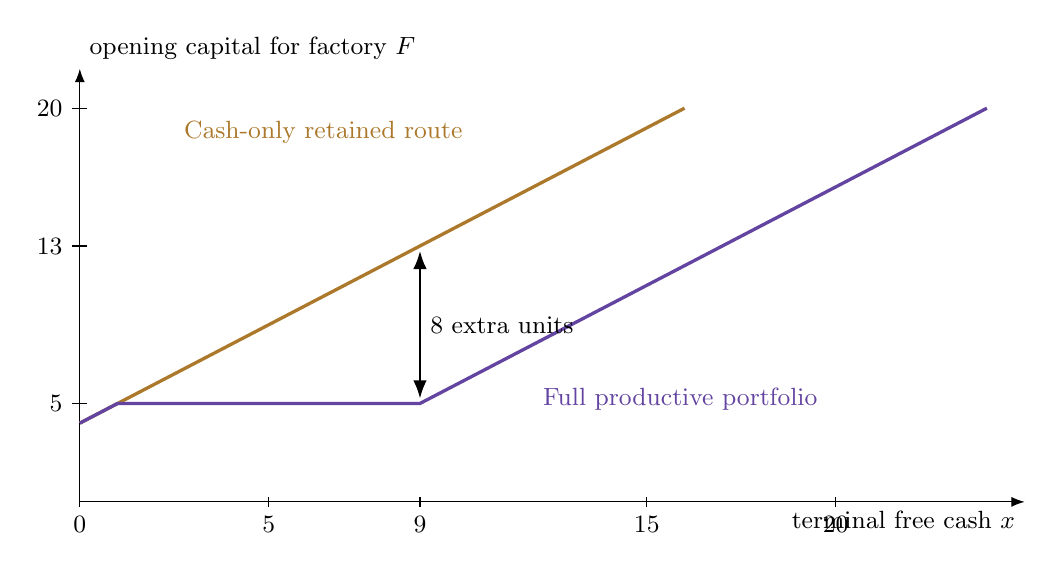
\begin{tikzpicture}[>=Latex,x=.48cm,y=.25cm,font=\small]
\draw[->] (0,0)--(25,0) node[below left]{terminal free cash $x$};
\draw[->] (0,0)--(0,22) node[above right]{opening capital for factory $F$};
\foreach \x in {0,5,9,15,20}{\draw (\x,.25)--(\x,-.25) node[below]{\x};}
\foreach \y in {5,13,20}{\draw (.2,\y)--(-.2,\y) node[left]{\y};}
\draw[very thick,gold] (0,4)--(16,20);
\draw[very thick,accent] (0,4)--(1,5)--(9,5)--(24,20);
\draw[<->,thick] (9,5.25)--(9,12.75) node[midway,right]{8 extra units};
\node[align=left,anchor=west,text=gold] at (2.5,18.8) {Cash-only retained route};
\node[align=left,anchor=west,text=accent] at (12,5.2) {Full productive portfolio};
\end{tikzpicture}
\caption{For target $F$, the cash-only response is $x+4$. The full response is $\min\{x+4,\max(5,x-4)\}$. The maximum gap is eight, attained at the critical target nine and beyond. The construction of $F$ is charged, not capitalized into imaginary spendable cash.}
\label{fig:cash}
\end{figure}

\subsection{Safe compression and one resource witness}
A retained $b$ covers $a$ at allowance $\varepsilon\ge0$ exactly when
\begin{equation}
 \kappa_b\le\kappa_a+\varepsilon,\qquad
 \delta_b\ge\delta_a+\rho(K_b,K_a)-\varepsilon.
 \label{eq:cover}
\end{equation}
Theorem~\ref{thm:main} makes covering every full producer equivalent to the uniform portfolio guarantee. A finite cover algorithm may select representatives, but each retained witness must include the executable reconstruction path and its current validity. The implementation computes exact losses for supplied subportfolios and removes only operationally dominated producers; it does not claim a new minimum-cardinality covering algorithm.

Successive substitution allowances add. Indeed the triangle for $\rho$ gives $d(a,c)\le d(a,b)+d(b,c)$: seed differences telescope, and the return difference plus reconstruction costs is bounded by the corresponding sum. A chain of deletions must retain its cumulative allowance or recompute a tighter direct bound.

For several resources, one must preserve one actual repair path. A path costing $(0,5)$ and another costing $(5,0)$ do not provide a repair costing $(0,0)$. Neither fits budget $(1,1)$. Money, machine occupancy and energy cannot be exchanged by taking coordinatewise minima. The scalar theorem does not solve multidimensional production, concurrency or physical resource conversion; those require compatible vector path semantics and the same-witness discipline of the earlier papers \cite{strategise,previous}.

\section{A digital foundry whose products participate in later construction}
\label{sec:foundry}
The preceding theorem admits supplied construction contracts. To avoid making every valuable dependency an unexplained label, the new reference constructs actual digital artifacts and derives the charges of its seven-capability production catalogue from their recorded search and checking work.

The foundry operates over rational vectors indexed by the binary group $G=(\mathbb Z_2)^k$, with $n=2^k$. This domain is chosen because linearity and bilinearity make complete finite certificates possible. It does not define the enterprise's ultimate product market. Transform generation and the underlying harmonic analysis are established \cite{spiral,odonnell}; the experiment is a vehicle for testing productive inheritance, not a claim to rediscover those methods.

\subsection{First product: a checked interaction transform}
The supplied specification is the Walsh matrix
\begin{equation}
 W_n[i,j]=(-1)^{\pop(i\,\&\,j)},\qquad (F_nx)_i=\sum_{j=0}^{n-1}W_n[i,j]x_j.
 \label{eq:walsh}
\end{equation}
The constructor starts with the one-element identity. Given a checked $F_{n/2}$, it enumerates 64 candidate compositions: two input layouts (halves or alternating coordinates), two output layouts (blocks or interleaving), and sixteen signed $2\times2$ mixing matrices. Each candidate invokes the retained child on the two input parts and mixes corresponding outputs. Its expanded coefficient matrix is compared with \eqref{eq:walsh}. Failed candidates, not just the winner, are saved and charged.

The selected realization has the familiar form
\begin{equation}
 F_n(x_L,x_R)=\big(F_{n/2}x_L+F_{n/2}x_R,\ F_{n/2}x_L-F_{n/2}x_R\big).
 \label{eq:butterfly}
\end{equation}
It performs $T(n)=2T(n/2)+n=n\log_2n$ arithmetic operations in the stated model. The family is constructed at sizes $2,4,8,16,32$, not loaded as precompiled transform artifacts. The target matrix, split/mix grammar and conventional factorization opportunity are supplied. A specialist can write \eqref{eq:butterfly} directly; neither invention of the Walsh algorithm nor a superior search policy is demonstrated.

The artifact is an ordinary JSON abstract syntax tree with dimensions, dependency identity, layout, mixing coefficients, a matrix certificate and an operating-work bound. It is interpreted by a restricted local evaluator. No generated Python source is passed to \texttt{eval} or \texttt{exec}, and no provider or external system is called.

\subsection{Second product: composition of independent effects}
The next target is binary-group convolution,
\begin{equation}
 (x\star y)_i=\sum_{j=0}^{n-1}x_jy_{i\oplus j}.
 \label{eq:conv}
\end{equation}
For probability vectors it gives the distribution of the XOR combination of two independent binary error patterns. It is not ordinary cyclic convolution under addition modulo $n$; the negative-control test distinguishes these operations.

The supplied programme template composes retained transforms with pointwise multiplication and a final normalization:
\begin{equation}
 C_n(x,y)=\frac1nF_n\big((F_nx)\odot(F_ny)\big).
 \label{eq:conv_program}
\end{equation}
The constructor tries four signed normalization candidates. An anchor input selects a candidate, but does not certify it. A separate checker evaluates all $n^2$ input basis pairs and verifies the complete output against $e_i\star e_j=e_{i\oplus j}$. Only then is the capability admitted. At $n=32$, the programme takes $3n\log_2n+2n=544$ arithmetic operations under the explicit model.

The fact that the constructor supplies this template is disclosed. The output is a correct instantiated programme and a checked dependency, not an autonomous discovery of the convolution theorem. The substantive inheritance is that the program calls the actual retained transform and its qualification applies to that content identity.

\subsection{Third product: an inverse whose checking uses a predecessor}
Fix a known rational kernel $h$. Let $M_hx=h\star x$. When every entry of $F_nh$ is nonzero, the constructed inverse is
\begin{equation}
 S_h(y)=\frac1nF_n\left((F_ny)\oslash(F_nh)\right).
 \label{eq:inverse}
\end{equation}
Here $\oslash$ denotes coordinatewise division. The reference uses $n=32$ and $h=(33,1,\ldots,1)$. Its spectrum is $64$ in the constant coordinate and $32$ in the other coordinates. The constructor calculates it from the retained transform, rejects singular kernels, and emits an inverse program with its explicit kernel and spectrum.

Qualification checks $M_hS_h(e_j)=e_j$ for every $j$. There are two legitimate architectures. The direct checker evaluates the defining convolution with $2n^2-n$ arithmetic operations per basis vector. The inherited checker uses the already qualified $C_n$ with 544 operations. Both execute the same inverse and compare all 32 output coordinates. Neither skips the requirement that the composed operator be the identity.

\begin{proposition}[Complete certificates in the declared arithmetic grammar]
\label{prop:basis}
A linear candidate equals its specified linear operator on all rational inputs if and only if it agrees on all input basis vectors. A bilinear candidate equals its specified bilinear map if and only if it agrees on all ordered basis pairs. In particular, checking $M_hS_h(e_j)=e_j$ for every $j$ certifies the inverse identity on all rational vectors when both programs have their stated linear meanings.
\end{proposition}
\begin{proof}
Write any vector as a linear combination of the basis and distribute the candidate and specification through that combination. For the bilinear claim, expand both arguments, producing a sum over ordered basis pairs. For the inverse identity, apply the linear claim to $M_hS_h$ and the identity operator. These arguments require the restricted grammar's linear or bilinear semantics; finite test agreement does not certify arbitrary unrestricted code.
\end{proof}

The checker is separately implemented and does not import the construction routine. The complete package also reruns the inverse check using direct convolution, so its qualification is not supported only by a chain sharing the generated transform. Those additional research checks are recorded separately from the selected deployment qualification charge. Both implementations share authorship; this is implementation diversity, not external peer review or proof-assistant verification.

\begin{figure}[htbp]\centering
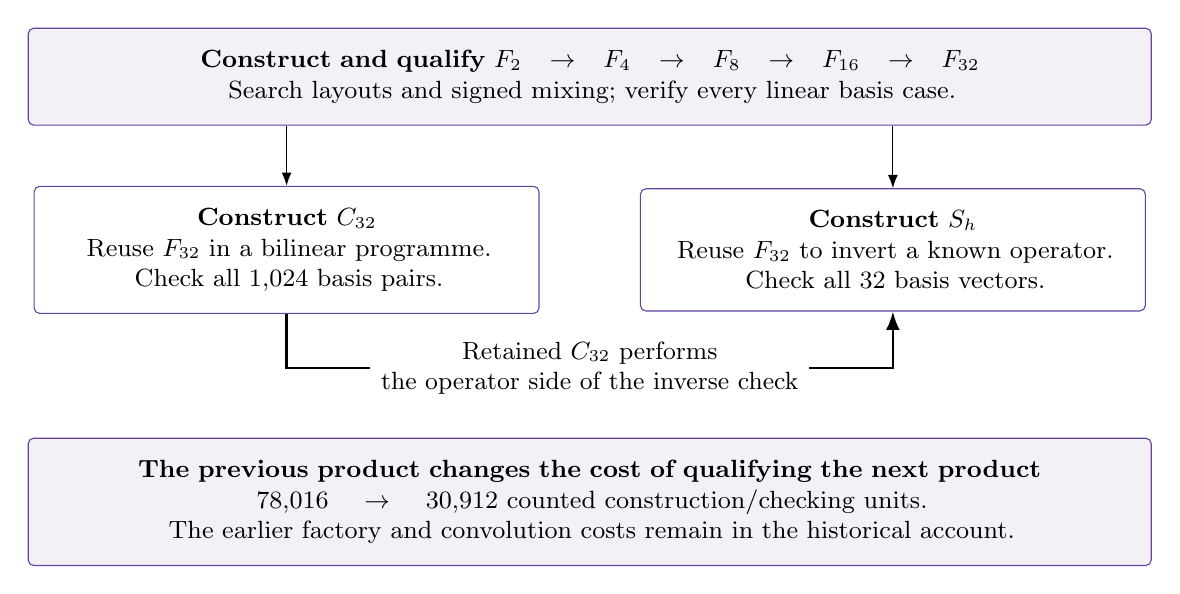
\begin{tikzpicture}[>=Latex,font=\small,
 box/.style={draw=accent,rounded corners=2pt,align=center,inner sep=8pt}]
\node[box,fill=pale,text width=13.7cm] (f) at (0,0) {\textbf{Construct and qualify $F_2\to F_4\to F_8\to F_{16}\to F_{32}$}\par Search layouts and signed mixing; verify every linear basis case.};
\node[box,text width=5.85cm] (c) at (-3.85,-2.2) {\textbf{Construct $C_{32}$}\par Reuse $F_{32}$ in a bilinear programme.\par Check all 1,024 basis pairs.};
\node[box,text width=5.85cm] (s) at (3.85,-2.2) {\textbf{Construct $S_h$}\par Reuse $F_{32}$ to invert a known operator.\par Check all 32 basis vectors.};
\draw[->] (f.south -| c.north)--(c.north);
\draw[->] (f.south -| s.north)--(s.north);
\draw[->,thick] (c.south) --(-3.85,-3.7)--(3.85,-3.7)--(s.south);
\node[align=center,fill=white,inner sep=4pt] at (0,-3.7) {Retained $C_{32}$ performs\\the operator side of the inverse check};
\node[box,fill=pale,text width=13.7cm] at (0,-5.4) {\textbf{The previous product changes the cost of qualifying the next product}\par $78{,}016\to30{,}912$ counted construction/checking units.\par The earlier factory and convolution costs remain in the historical account.};
\end{tikzpicture}
\caption{An executed productive dependency, not an asserted asset valuation. The mathematical templates and domain are supplied. Generated artifacts, their complete basis checks and the changed qualification work are actual outputs.}
\label{fig:foundry}
\end{figure}

\section{Price the work that was actually performed}
\label{sec:work}
\subsection{A declared operational metric}
Each recorded specification cell, candidate record, coefficient operation, coefficient comparison, rational arithmetic operation and verification comparison costs one \emph{work unit}. Addition, subtraction, multiplication, division and an explicit sign negation each count as one. Indexing, allocation, serialization, hashing and control overhead are not included. Rational numerator/denominator bit growth is also not charged; this is an arithmetic-count model, not bit complexity or processor time.

Failed candidates are charged. Qualification is charged. Retained artifacts are charged when constructed, once per actual history. Additional checking done for this research is counted separately rather than used to suggest that the full research campaign was cheaper. Authoring, mathematical invention, literature review, engineering, actual energy, independent institutional review and commercialization were not comprehensively metered. Their costs are unmeasured, not zero.

For $n=2^k>1$, the transform-construction charge is
\begin{align}
 B_F(n)&=n^2+64+64n^2+64n^2\notag\\
       &\quad+n(n\log_2n)+2n^2\notag\\
       &=(131+\log_2n)n^2+64.
 \label{eq:buildF}
\end{align}
The first line records the specification and all candidate coefficient work. The second records every basis execution plus matrix/output comparison. The separately implemented checker derives the candidate validity again by forward interpretation of every basis, rather than trusting the compiler's matrix expansion.

\begin{table}[htbp]\centering\small
\caption{The entire retained transform chain. Parent costs are inherited, not repeatedly hidden or newly expensed at every row.}
\begin{tabular}{@{}lrrr@{}}\toprule
Artifact & New build and qualification & Cumulative charge & Per-use arithmetic\\\midrule
$F_2$ & 592 & 592 & 2\\
$F_4$ & 2,192 & 2,784 & 8\\
$F_8$ & 8,640 & 11,424 & 24\\
$F_{16}$ & 34,624 & 46,048 & 64\\
$F_{32}$ & 139,328 & 185,376 & 160\\\bottomrule
\end{tabular}
\label{tab:chain}
\end{table}

At $n=32$, the convolution's candidate construction costs 2,308 units. Checking 1,024 basis pairs costs
\begin{equation}
 1{,}024(544+32)=589{,}824,
\end{equation}
so its added construction charge is 592,132. These are intentionally conservative full-basis checks. A specialist exploiting a symbolic compositional proof can qualify the same operator more cheaply. The reported optimum later is relative to the implemented construction and checking recipes, not every possible formal proof.

The inverse's spectrum and artifact preparation cost 192. Its direct and inherited qualification charges are respectively
\begin{align}
 32(384+2{,}016+32)&=77{,}824,\\
 32(384+544+32)&=30{,}720.
\end{align}
Adding 192 gives 78,016 and 30,912. Exactly 47,104 counted operations are avoided because a previously certified operator replaces the direct reference implementation. There is no change in required output, number of checked basis vectors or admitted rational domain.

\subsection{A stronger comparison is allowed to tie}
The transform's direct signed summation needs $n(n-1)=992$ additions/subtractions at $n=32$ if each output starts with its first term. Direct convolution needs $2n^2-n=2,016$ arithmetic operations. The foundry's selected transform, convolution and inverse use 160, 544 and 384, respectively. These are classical operation-count reductions, not measured Python speedups or state-of-the-art signal-processing records. SPIRAL already generates optimized transform code and searches representation and implementation choices \cite{spiral}. Its hardware-tuned code is not benchmarked here.

Likewise, an unrestricted planner with the same construction graph obtains the same joint solution. The diagnostic isolated-build comparison reconstructs the transform chain separately for each of three products and verifies the inverse directly. Its charge is
\begin{equation}
 3(185{,}376)+592{,}132+78{,}016=1{,}226{,}276.
\end{equation}
A shared construction pays
\begin{equation}
 185{,}376+592{,}132+30{,}912=808{,}420.
\end{equation}
The 417,856-unit difference consists of two avoided transform rebuilds (370,752) and the improved inverse qualification (47,104). The comparison isolates a dependency structure. It does not establish that existing compilers or competent engineering teams normally repeat all this work.

\subsection{A tool is not worth building merely because it can help}
If only the inverse is required and $F_{32}$ already exists, the correct route costs 78,016. Building $C_{32}$ first would cost $592{,}132+30{,}912=623{,}044$. The 47,104-unit checking saving alone does not pay for that construction. The exact planner selects the direct route.

If the convolution is also an accepted required output, or is genuinely inherited from a prior useful mission, its construction has a separate purpose. Then the inverse can use it for 30,912 additional units. This is the difference between legitimate productive inheritance and inventing extra work to make a compounding story look attractive. A sunk artifact is not free historically; its cost is common to the continuation comparison only when it really has already been obtained.

\section{The generated artifacts support materially different uses}
\subsection{Interaction analysis}
The transform is applied to the supplied scalar function on five binary choices,
\begin{equation}
 f(x)=3+2\chi_1(x)-\chi_6(x)+\tfrac12\chi_{24}(x),\qquad
 \chi_j(x)=(-1)^{\pop(x\,\&\,j)}.
\end{equation}
The normalized output $F_{32}f/32$ has exactly four nonzero coefficients, at indices $0,1,6,24$, with values $3,2,-1,1/2$. The application recovers those interactions. The function is authored, not a newly discovered scientific law; the artifact realizes a complete rational-vector transform rather than a lookup for that one function.

\subsection{Composition of independent binary disturbances}
The convolution combines a distribution with mass $1/2$ at $0,1$ and one with mass $1/4$ at $0,2,4,6$. It returns a nonnegative unit-mass distribution, checked against the direct definition. This is a bilinear operation on two independently supplied distributions, not a renamed transform query. Independence is an input premise; a joint distribution with correlated effects would require another model.

\subsection{Inverse reconstruction}
A third application supplies the known kernel $(33,1,\ldots,1)$ and observations of its action on a rational vector with coordinates $((7i+3)\bmod13)/13$. The constructed inverse recovers every coordinate exactly. This is an inverse problem with a known operator and exact arithmetic. It does not infer an unknown physical mixing law, establish conditioning in floating point or perform experimental calibration.

Across the three applications, 96 scalar outputs are independently checked. A fresh fixed-seed block adds 100 vector cases across sizes 2,4,8,16,32. At size 32 it also executes convolution and inverse reconstruction, yielding 140 vector checks and 2,520 scalar comparisons. The complete-basis argument, not the number of sampled cases, supplies the all-rational-input guarantee within the grammar.

\section{One enterprise state for construction, funding and continued use}
\label{sec:finance}
The retained enterprise state is not reduced to a financial account. It includes qualified artifacts, executable construction recipes, validity and resource contracts, observed receipts, reserves, obligations and current authority. The scalar theorem is a projection of that state at a compatible, reserve-closed boundary. It is not permission to drop a field that later affects what can be executed.

A qualified callable endpoint carries its linked implementation dependencies. The logical stock records separately available, certified interfaces, not every private subroutine byte. An imported endpoint does not automatically grant an exported contract or usage right for every internal component; those must be qualified separately. The actual generated sequence exports and retains its ancestors.

The new construction graph contains seven types: $F_2,F_4,F_8,F_{16},F_{32},C_{32},S_{32}$. Its eight recipes are the five transform extensions, the convolution, and two inverse checking architectures. Costs are taken from the observed work ledgers. The minimum all-three-product route costs 808,420. Every one of the $128\times128=16,384$ formal stock--target completion values is checked by the independent dynamic programme. Arbitrary masks are comparison contexts under the supplied type semantics, not claims that all corresponding hardware or packaging configurations have been separately deployed.

This changes what \emph{Out-Think} must preserve: not merely cash and a success flag, but the executable dependencies that make successor costs different. It changes \emph{Out-Strategise}: compare whole producers using \eqref{eq:dominance}, not terminal profit alone. It changes \emph{Out-Evolve}: the transition must actually add a usable function or lower a justified construction requirement, rather than just increase an internal asset score.

\subsection{A derived funding boundary instead of an invented customer}
No sale occurred in this study. To examine financing without fabricating demand, suppose a hypothetical service provider charges one work-credit unit per counted construction unit. This tariff covers only the defined work subtotal; additional real-world costs must be priced separately before making a business claim.

Let $K=185{,}376$ fund the checked transform chain and $H=592{,}132$ fund the convolution using that inherited chain. Start with $K$, spend it on the first accepted construction, receive an actually available payment $P$ under the hypothetical terms, and then construct the successor. Preserving the original principal requires
\begin{equation}
 P-H\ge K\quad\Longleftrightarrow\quad P\ge K+H=777{,}508.
 \label{eq:funding}
\end{equation}
A smaller $P\ge H$ may finance the successor while consuming principal. A promised but unpaid $P$ finances neither. The test cases include zero payment, mere cost recovery, one unit below the principal-preserving boundary, the boundary and one unit above. The threshold is derived from executed work counts; it is not an estimate of willingness to pay or an assertion that these tools merit that price.

For a real programme, let $P$ be receipts after current obligations, $K$ fully priced first construction and $H$ the qualified successor's complete remaining requirement. Research effort, failed discovery, independent checking, delivery, support, financing, taxes and capacity must be accounted for consistently. Equation~\eqref{eq:funding} remains simple arithmetic, not a theorem that customers will create the required margin. \emph{Invent the Economy} makes the technical construction, beneficiaries, accepted arrangement, rights and financing a joint object of investigation \cite{economy}.

\subsection{What the enterprise would sell and retain}
The proposed product is a qualified computational or scientific capability and a maintained construction path for its supported extensions. An actual sponsor might purchase bounded research, then separately accept a deployment with specified throughput, precision, supported domain and obligations. Real recurring fees must purchase maintenance, access, adaptation or requalification, not preserve work that the invention makes unnecessary.

The foundry itself is not proposed as a novel market for basic Walsh software. Established mathematical libraries and generation systems are strong competitors. Its purpose is to expose a general enterprise decision: does retained productive structure materially lower the complete cost of a different useful capability? A commercially consequential instance would need an independently selected bottleneck, competitive alternatives, actual beneficiary evidence and a priced delivery plan.

MONTREAL.AI's parent ownership remains intact. Separate application ventures can be negotiated without granting automatic parent equity. Public algorithms remain public; code licenses, customer-specific data and agreed reuse rights determine what is legitimately retained. The AGIJobManager USDC route and Alpha/Jobs v0 \$AGIALPHA routes remain distinct in the proposed integration. Nothing in this manuscript creates dividends, ownership of infrastructure, equity claims or guaranteed token appreciation. Company resources and token valuation are not interchangeable.

\subsection{Current authority does not compound automatically}
A checked predecessor can help compute a new artifact. It cannot approve its own spending limit, sign a customer's acceptance, authorize publication or command a physical instrument. The architecture requires current approval for the actual action and resources. The new foundry performs only local computation; the inherited ledger's supplied authorization and replay controls remain software tests, not external authentication.

A hash binds an artifact to bytes. It does not establish its semantics. The checkers reject a deliberately wrong normalization even after its hash has been recomputed. They also reject a modified dependency, a false operating bound and use of an unqualified predecessor as a reference. Qualified inheritance is a chain of applicable evidence, not a chain of self-issued labels.

\section{Executed confirmation, failures and preserved evidence}
\subsection{What was frozen and what was tested}
The final new run uses seed 20261021817. Its source identities are recorded before generating confirmation. The author chose the model family and protocol, so this is not externally blinded evaluation or preregistration.

Seventy-two finite catalogues contain three to five capabilities. Each has standalone recipes ensuring complete reconstruction plus joint or prerequisite-dependent recipes, some with zero nonnegative charge. Their possible producer policies have different output stocks and valid seed/gain pairs. The reference verifies all completion entries, compares the retention formula with direct target scans and checks the theorem's critical witness. Productive-dominance pruning has zero observed loss in every case.

\begin{table}[htbp]\centering\small
\caption{New executed evidence. Counts refer to finite computations, not independent enterprises or scientific discoveries.}
\begin{tabularx}{\linewidth}{@{}YrY@{}}\toprule
Check & Count & What it establishes\\\midrule
Generated construction catalogues & 72 & Supplied optional-capability class\\
Generated stock--target completion values & 32,256 & Two exact solvers agree\\
Capability/cash targets scanned & 28,472 & Exact retention identity and witnesses\\
Triangle checks in the first twelve catalogues & 149,504 & Operational completion property\\
Foundry stock--target values & 16,384 & Minimum cost under measured recipe charges\\
Transform candidate programmes & 320 & Complete specified search; 12 valid candidates\\
Selected artifact basis cases & 1,118 & Complete linear/bilinear-domain checks\\
Additional direct inverse basis cases & 32 & Alternate checking implementation\\
Candidate coefficient checks & 87,296 & Independent replay of all transform candidates\\
Fresh vector/scalar comparisons & 140 / 2,520 & Exact evaluated outputs\\
Distinct-application scalar comparisons & 96 & Interaction, convolution and inverse uses\\
New unit-test methods & 51 & Boundaries, mutations and negative controls\\\bottomrule
\end{tabularx}
\label{tab:counts}
\end{table}

The scan covers all target stocks and integer cash targets through a bound beyond every response breakpoint. Integer profile and reconstruction costs make all breakpoints integral; beyond the final breakpoint all responses have slope one and the difference is constant. This finite computation checks the formula in these instances. The continuous-target and arbitrary-family statements rest on the proofs.

\subsection{Failures that the enterprise must not relabel as progress}
\paragraph{A noncomposable cost table.}
A supplied table has $\rho(L,K)=1$, $\rho(K,Q)=1$ and $\rho(L,Q)=5$. For equal zero-cash producers leaving $K$ and $L$, the pairwise shortcut predicts one, but keeping only $L$ has actual loss four at $Q$. The missing two-unit concatenated path means the table is not the operational completion function claimed by the theorem. The study records the failure rather than declaring the shortcut universally valid.

\paragraph{Unseeded production cycles.}
A recipe makes $a$ from $b$ and another makes $b$ from $a$. Starting with neither, no construction is available. A directed cycle in a dependency diagram is not self-production. Exhausted reachable-stock search supplies the obstruction. A state cap supplies only an incomplete result.

\paragraph{Wrong group, wrong capability.}
For a point mass at index one, XOR convolution with itself returns a point mass at zero. Ordinary cyclic convolution returns index two. The same-looking input/output dimensions do not license substituting one group law for the other. New semantics require a new certificate.

\paragraph{Singular or numerically different operation.}
A constant kernel has zero nonconstant Walsh components and no full inverse; the constructor rejects it. Exact rational correctness is not a finite-precision stability result. A floating-point implementation, overflow limit or noisy application must receive its own error contract and cannot inherit exactness by file name.

\paragraph{Verification and finance failures.}
Changed mixing coefficients, altered divisors, an incorrect inverse spectrum, missing parents and insufficient operation limits fail checking. A reconstructed hash does not repair them. Fully reserved research money cannot fund the factory while its refund remains protected. An unreceived payment cannot be counted as a receipt. These controls address different obligations; one passing check does not satisfy the others.

\subsection{The earlier contribution is preserved and reproduced}
The supplied 24-page edition remains unchanged in the companion. Before the new work, its code was inspected and rerun. All forty tests passed; ten deterministic outputs matched their supplied originals byte-for-byte. The rerun preserved its 64 contract graphs, 41,664 budget--target comparisons, 256 portfolio cases, nine computational deliverables and modeled three-batch cash record. Those are \emph{reproduced inherited results}, not additional new experiments of this revision.

The original capital theorem remains the equal-stock case of Theorem~\ref{thm:main}. Its observed DAG compiler, reserve accounting and local ledger are not replaced by the new pure-expense reconstruction graph. They occupy different layers. A producer can contain receipts, failures and timed reserves; the repair summary used here has the narrower stationary nonnegative-cost semantics.

\section{From productive inheritance to larger productive systems}
\label{sec:scale}
The bounded foundry suggests a precise unit of expansion. For a qualified stock $K$ and a resource budget $B$, define
\begin{equation}
 \mathcal G_B(K)=\{Q:\rho(K,Q)\le B\}.
 \label{eq:frontier}
\end{equation}
This is a construction frontier, not a list of ideas or a valuation. A predecessor matters when an actually retained capability lets a later target enter that frontier, or reduces its required resource while preserving all material obligations. Adding a label without executable scope does neither.

The inverse example supplies a strict finite instance. Once the transform and convolution are validly inherited, a 30,912-unit construction allowance reaches the new inverse under the inherited checking architecture. With the transform alone it does not: the cheapest available recipe needs 78,016. The earlier cost of acquiring the convolution remains in the historical campaign. This is productive leverage under a declared resource comparison, not free wealth.

At larger scales, an enterprise would seek tools that change the construction frontier itself: a better experiment that shortens qualification, a production interface that permits independent modules, a manufacturing method that reduces the material needed for another machine, or an energy system that supplies a larger reliable operating budget. Those are research targets, not consequences already proved by a small digital example.

\subsection{A sequence with real intermediate obligations}
A credible expansion begins with a computational capability whose outputs can be accepted independently. It proceeds to a scientific instrument only after hardware, calibration and operating evidence exist. A pilot production system must establish manufacture, maintenance and useful throughput. Energy and industrial infrastructure require actual land or access, materials, conversion efficiencies, safety, finance and competent operation. Space-based productive systems add transport, thermal management, fabrication and maintenance requirements. No paper, ledger valuation or internal token transfer supplies these assets.

The intended long-horizon enterprise is a growing network of mutually useful instruments and productive facilities. Some capabilities supply knowledge; others create manufacturing options, lower verification cost, or expand resource availability. Their coordination should be evaluated by accepted external output and the construction frontier left afterward. An expanding agent population alone is not that network.

The same logic forbids an automatic exponential forecast. Demand may saturate. A newly admitted tool may be redundant. Qualification, upkeep or integration may dominate savings. A facility can become the new bottleneck, and concurrent users may require a capacity model that the optional-set abstraction lacks. A path can be financeable but not socially or commercially worthwhile. The enterprise must retain the option not to build.

\subsection{The decisive next empirical study}
The next natural experiment should select a public-input technical requirement independently of this foundry. It should allow a strong specialist, an unrestricted agent and the proposed system to reuse, generate, verify and redesign under comparable total resources. The initial primitives and previous artifacts must be matched or explicitly priced. At least one genuinely different later task should be withheld from construction selection.

Record separately: the delivered artifact, complete discovery and checking effort, actual reuse, cost of reconstructing the missing tool in an ablation, and acceptance of the successor. A business extension additionally requires real participant consent, delivered obligations, observed receipts and available funds. A generator's improvement should be tested across independent campaigns; a richer starting toolbox is not evidence that its invention policy learned. This experiment remains unrun. It is a specific next test, not a substitute for the completed finite construction.

\section{Nearest prior art and what is actually new}
\subsection{Generated software and inherited checking}
SPIRAL generates implementations of signal-processing transforms through mathematical representations, formula generation, translation and search \cite{spiral}. Its scope and performance engineering are considerably broader than the reference here. The present work does not originate recursive transforms, factorization search or libraries that generate code. Standard Boolean harmonic analysis supplies the Walsh characters, convolution diagonalization and inverse formulas \cite{odonnell}.

Certifying algorithms produce witnesses whose checking can be simpler than generation; verification of those checkers is itself a separate obligation \cite{certifying}. Our complete-basis checks exploit a restricted exact grammar. They are not formally verified checkers in VCC or Isabelle, and they do not certify arbitrary LLM-generated programs. The new experimental role is to make a retained checked operator participate in another operator's qualification, then connect the measured reconstruction difference to enterprise succession.

\subsection{Resources, portfolios and constructive substitution}
Automatic amortized resource analysis gives a formal account of resource high-water marks and returned resources \cite{kahn}. Shortest paths compute minimum sums over nonnegative construction transitions \cite{dijkstra}. The previous enterprise paper supplies the capital-response portfolio result for equal output types \cite{previous}. The revised \emph{Out-Strategise} gives continuation guarantees for alternative capability sets with submodular acquisition costs \cite{strategise}.

The new theorem joins these ideas at a different boundary: producers can leave \emph{different} stocks, and replacement depends on an executable cost of rebuilding the predecessor's productive means. The exact critical target includes both that stock and its available closing cash. The triangle is sufficient and universally necessary within the stated class of completion maps. This is a specific extension, not a claim to originate directed distances, program composition, enterprise finance or every related retention result. The literature review is focused, not an exhaustive priority proof.

\subsection{Contemporary agent research is context, not a defeated baseline}
AlphaEvolve develops executable algorithms through model-generated changes and evaluation-driven search \cite{alphaevolve}. It may supply candidate constructors or optimizations; it is not assumed unable to reframe or build tools. Vending-Bench evaluates sustained operation in a simulated business \cite{vending}; its balances are a different evidence category from accepted external revenue. AhaBench examines whether experience becomes reusable capability across changing tasks and long-horizon settings \cite{aha}. We inspected its stated benchmark design, not independently reproduced its results.

These sources support taking generation, persistent operation and transfer seriously as separate empirical questions. The reference here makes no model-provider calls and does not report a head-to-head advantage. An unrestricted exact planner matches the constructed optimum. The proposed distinction is a verified productive inheritance and an exact account of what losing it can cost, not a universal intelligence ranking.

\section{Conclusion: retain what can build the next capability}
A business can complete its present task, collect more cash, and still leave the next mission less attainable. Cash matters, but so do the qualified means that determine how much cash a future construction needs. The relevant inheritance is a joint object.

This revision makes that object concrete. A digital foundry constructs and checks a transform, a convolution operator and an inverse. The retained convolution changes the actual work needed to qualify the inverse. A finite operational construction graph turns those consequences into successor requirements. An exact capital--capability theorem determines how much deleting an alternative producer can add to any declared successor's launch capital, and identifies a single attaining target. Its boundary is executable concatenability, not a presumption that all costs are submodular.

The founding hierarchy remains intact. AGI ALPHA organizes accountable work. Transformational intelligence changes unnecessary constraints. The six stages produce evidence, representations, constructions, alternatives, accepted execution and checked evolution. \Om{} inherits the means that remain valid, not an automatic right to spend or a fictional balance-sheet value.

\thesis{\centering\large\textbf{Don't just build intelligence.\\Build what intelligence can become.}\par\medskip
\normalsize Build the means of building. Preserve what makes the next capability attainable.\par\smallskip
\textbf{Find your Alpha. Build your SUCCESSOR $\Omega$.}}

\paragraph{Research status.} This is an AI-assisted mathematical and software manuscript. Its new experiments are exact rational, integer and finite-model computations with authored tasks and cost conventions. The mathematical proofs are written arguments, not proof-assistant formalizations. Separate implementations share authorship. No physical deployment, autonomous discovery of primitive laws, market adoption, actual revenue, external peer review or superior learned discovery policy is claimed. The original manuscripts, repository, deployed systems, wallets and permissions remain unchanged.

\appendix
\section{Proof details and interpretation of the boundary}
\subsection{Why the repair charge is a real continuation}
A cost for missing capabilities is meaningful only if a competent builder can follow its path. The output witness records initial stock, required target, selected recipe, paid charge and next stock at every step. A checker rejects an unmet prerequisite or a mismatch between the declared output and the stock transition. For an unreachable target, a complete reachable set must contain the initial stock, be closed under every admitted action and contain no stock covering the target. A capped search cannot emit that certificate.

An optimal path need not produce exactly $Q$. A package may create extra capabilities cheaply; optionality permits retaining them without forcing their use. The minimum in \eqref{eq:rho} therefore ranges over every final stock \emph{containing} $Q$. Requiring exact equality would incorrectly penalize a useful byproduct and can break the intended triangle.

The theorem applies to any finite complete subdomain with the stated triangle, not only all subsets of a large catalogue. If a retained producer cannot reconstruct a required full output, an infinite loss may occur. The code reports an unbounded-missing-capability status rather than subtracting infinities. Finite guarantees require either a finite fallback for the relevant domain or a narrower explicitly admitted target set.

\subsection{Exact single-policy substitution and signed differences}
For fixed $a,b$, \eqref{eq:upper} shows that the difference of their capital response functions is at most $d(a,b)$. The critical successor $(K_a,\kappa_a+\delta_a)$ attains it exactly. Thus $d(a,b)$ is the exact worst directed response difference. It can be negative when $b$ is uniformly better, even though reconstruction charges are nonnegative.

For a retained subportfolio, $F_\B\ge F_\A$ at every target. The maximum--minimum expression in Theorem~\ref{thm:main} must consequently be nonnegative. No artificial clipping is necessary. A family with several equivalent producers may keep a stable representative. The implementation removes a producer only when another dominates it operationally; in equivalent classes it retains the earliest representative. Transitivity of the directed substitution inequality prevents a cycle of strict improvements from deleting every member.

For composition, the two defining coordinate differences each obey their respective telescoping bound. In particular,
\begin{equation}
 \delta_a-\delta_c+\rho(K_c,K_a)
 \le[\delta_a-\delta_b+\rho(K_b,K_a)]
    +[\delta_b-\delta_c+\rho(K_c,K_b)].
\end{equation}
Both bracketed terms are bounded by the corresponding $d$, and the seed difference also telescopes. This proves the stated substitution triangle. It is not a theorem that changed prices, rights or clocks preserve an old certificate.

\subsection{What cash profiles leave outside the summary}
The producer's guaranteed gain may occur on a different branch from its peak capital requirement; both are still universal guarantees of the same contingent policy. If output capability differs by branch, the summary must retain that branch-dependent stock or use a genuinely common weaker output type. Replacing such a family with its best stock from one branch and its best cash from another is invalid.

Similarly, a completion recipe with speculative revenue is not a pure expense. One may represent it using the previous edition's capital--return path semantics, but its endpoint resources and capability conditions must compose. The present theorem does not provide an unproved shortcut for cyclic companies, infinitely renewed customers, endogenous credit or hidden liability tails.

\section{Exact operator mathematics and checking scope}
\subsection{The three identities, with their classical source}
For $a,b\in G$, character orthogonality gives
\begin{equation}
 \sum_{x\in G}(-1)^{a\cdot x}(-1)^{b\cdot x}
 =\begin{cases}n,&a=b,\\0,&a\ne b.\end{cases}
\end{equation}
If $a\ne b$, pair each $x$ with $x\oplus e_j$ at a differing coordinate; the signs cancel. Consequently $W_n^2=nI$. Also,
\begin{align}
 [F_n(x\star y)]_a
 &=\sum_{i,j}(-1)^{a\cdot i}x_jy_{i\oplus j}\notag\\
 &=\left(\sum_j(-1)^{a\cdot j}x_j\right)
   \left(\sum_k(-1)^{a\cdot k}y_k\right).
\end{align}
This proves \eqref{eq:conv_program}; division by nonzero transformed kernel entries proves \eqref{eq:inverse}. These are established Fourier identities on a binary group \cite{odonnell}, proved here to state exactly what the implementation and transfer assume.

The inverse's kernel has one coefficient $n+1$ and $n-1$ coefficients one. Its constant transform component is $2n$ and every nonconstant component is $n$, so it is nonsingular. The constant-one kernel instead has only the constant transformed component; the missing components cannot be recovered by any full inverse. Its rejection is semantic, not a numerical tolerance decision.

\subsection{Why inherited checking is not circular}
$F_2$ is checked using a specification independent of its candidate-generation procedure. Each later $F_n$ is checked on every input basis, and its actual dependency bytes are bound into its AST. $C_{32}$ is then checked on every bilinear basis pair against the explicit XOR target, not against an assertion made by the inverse. Only after this does the inherited inverse checker use $C_{32}$. The dependency order has no cycle.

A new artifact cannot enter the qualified set merely because its hash is present. The package's topological verification establishes the predecessor's contract before its use. The direct inverse checker is an additional research control. For arbitrary executable code, basis tests alone would not prove linearity; here the restricted syntax and interpreter establish that property. Exact mathematical correctness also does not certify interpreter security in adversarial environments or a compiler outside this grammar.

\subsection{Runtime and construction counts are different denominators}
The selected recursive transform uses $n\log_2n$ arithmetic operations. Its convolution uses three transforms plus $n$ products and $n$ divisions; the inverse uses two transforms plus $n$ divisions by spectrum entries and $n$ normalization divisions. These give the operating counts 160, 544 and 384 at $n=32$.

Construction explores alternatives and checks them, so its cost is much larger. The complete transform chain costs 185,376 under \eqref{eq:buildF}. The quadratic number of complete convolution basis pairs contributes most of its 592,132-unit incremental cost. These numbers do not measure algorithmic novelty, model intelligence or an efficient industrial compiler. They make the specific inheritance comparison reproducible. Alternative proof architectures, hardware execution, sparse kernels, symbolic verification or stronger supplied primitives could reduce them.

\section{Inputs, implementation and independent replay}
\subsection{Finite construction confirmation}
Case $i=0,\ldots,71$ has $m=3+(i\bmod3)$ capabilities. Every singleton has a standalone recipe with cost drawn uniformly from integers two through fourteen. There are $m+3$ additional recipes: each prerequisite is independently included with probability .30, each produced capability with probability .38, with one produced capability forced when that draw is empty. Added recipe costs are uniform integers zero through ten. These are generator settings, not empirical frequencies.

There are $3+(i\bmod4)$ producers. Seed lies in $\{0,\ldots,10\}$, gain in $\{-\kappa,\ldots,14\}$ and output stock in all $m$-bit masks. A nonempty retained subfamily is drawn. The complete recipe, cost and producer tables are saved. Both solvers evaluate every stock--target cost. Direct cash-target scanning covers $x=0,\ldots,1+\max\kappa+\max\delta$. Since $\rho\ge0$, this upper limit exceeds every possible kink $\kappa+\delta-\rho$; after that point all candidate capital functions are linear.

The first twelve catalogues additionally receive every ordered triangle check. The new generated counts are not extrapolated to large industrial catalogues. The exact stock search has $2^m$ states, and the explicit completion table has $4^m$ entries. The implementation permits a state cap but makes no large-scale planning claim.

\subsection{Foundry and applications}
The source supplies the five transform sizes, coefficient specification, layout/mixing grammar, pointwise-product convolution template, signed divisor candidate set $\{-n,-1,1,n\}$, spectral inverse template and known kernel. Those are research inputs. Search produces the selected layouts and mixing, normalized programmes, spectra, complete certificate records and exact cost ledgers.

Fresh vector cases cycle through sizes 2,4,8,16,32. Coordinates are integers in $[-7,7]$; the second convolution argument at size 32 uses integers in $[-5,5]$. Inverse checks use the known kernel. All realized inputs and outputs are retained, so replay does not depend on regenerating a hidden random distribution. Separate application records contain all rational inputs and their exact outputs.

The source freeze occurs before confirmation generation. The first development block used seed 20261021811 and twelve catalogues. Its outputs remain preserved, but its earliest source was not separately archived; that directory is not advertised as a standalone reproducible historical release. A later review made explicit the research-funding trace in the cash counterexample, added operating-bound checks, checked the distinct application outputs independently, and added the nonsubmodular bulk-construction control. Final source and outputs are reproducible.

\subsection{Commands and artifacts}
The new study uses Python's standard library only. It does not install dependencies, call a provider, execute downloaded code, contact customers or transact. From the package root:
\begin{verbatim}
python code/run_research.py --out rerun --seed 20261021817 --cases 72
python code/check_research.py --results rerun
python -m unittest discover -s code -p 'test_*.py' -v
pdflatex -no-shell-escape -interaction=nonstopmode -halt-on-error \
  -output-directory=paper paper/Autonomous_Enterprises_Revised.tex
\end{verbatim}
Run the TeX command twice to settle references. The study refuses to overwrite a nonempty output directory. Scientific JSON and artifact identities are deterministic; platform and wall-clock metadata are separate. The LaTeX embeds its diagrams and bibliography. No fonts or external image files are redistributed.

\begin{table}[htbp]\centering\small
\caption{Principal new reproducibility files. The unchanged preceding package is included separately.}
\begin{tabularx}{\linewidth}{@{}P{.42\linewidth}Y@{}}\toprule
File & Role\\\midrule
\path{code/production.py} & Construction witnesses, productive dominance, capital--capability retention.\\
\path{code/reference_production.py} & Different completion recursion, direct target scans and path checking.\\
\path{code/foundry.py} & Candidate grammar, artifact generation and work accounting.\\
\path{code/verify_foundry.py} & Independent interpreter, direct operators and complete basis qualification.\\
\path{code/check_research.py} & Saved-output checking without either constructor import.\\
\path{code/test_revision.py} & Fifty-one tests, mutations and scope/funding controls.\\
\path{results/final/foundry.json} & All construction attempts, receipts, artifacts and measured work.\\
\path{results/final/foundry_plans.json} & Operational recipes, all completion values and four selected build paths.\\
\path{results/final/confirmation.json} & Seventy-two complete finite models and retention results.\\
\path{results/final/critical_example.json} & Cash-rich counterexample, realizing traces and witnesses.\\
\path{results/final/conditional_funding.json} & Symbolic tariff boundary cases; no actual receipts.\\
\path{provenance/} and \path{review/} & Source audit, original reproduction, logs and production review.\\\bottomrule
\end{tabularx}
\end{table}

\section{Claim--evidence register}
\small
\begin{longtable}{@{}P{.29\linewidth}P{.34\linewidth}P{.31\linewidth}@{}}\toprule
Claim & Evidence & Principal boundary\\\midrule\endfirsthead
\toprule Claim & Evidence & Principal boundary\\\midrule\endhead
Operational reconstruction satisfies a directed triangle & Proposition~\ref{prop:completion}; independent completion tables & Compatible, optional durable stock; stationary nonnegative recipe costs.\\[4pt]
Exact capital cost of retaining fewer producers & Theorem~\ref{thm:main}; 28,472 direct target checks & Same clean contractual boundary; finite reconstruction; unchanged tariffs and rights.\\[4pt]
Triangle is the exact universal boundary & Proposition~\ref{prop:boundary}; explicit invalid table & Universal finite reflexive maps; not a physical model-validation theorem.\\[4pt]
Cash-only dominance can discard a valuable factory & Five-versus-thirteen example with complete traces & Illustrative one-time payments and prices, not a real sponsor.\\[4pt]
Produced artifacts compute their declared functions & Complete linear/bilinear basis certificates & Exact rational syntax; no arbitrary-code or floating-point guarantee.\\[4pt]
A predecessor reduces successor qualification work & 78,016 versus 30,912 under two recorded checks & Declared arithmetic work, inherited qualification, no total-invention or market-price claim.\\[4pt]
Joint construction avoids duplicated work & 808,420 versus 1,226,276; independent path solver & Isolated-build ablation; unrestricted joint specialist matches.\\[4pt]
Prior enterprise study is preserved & Forty tests and ten deterministic output matches & Reproduced synthetic study, not newly observed revenue.\\[4pt]
Available receipts can fund another construction & Conditional threshold \eqref{eq:funding} and five cases & Hypothetical work-credit tariff; actual demand and funds unestablished.\\[4pt]
Larger productive systems can be built this way & Explicit research and business pathway & Physical qualification, materials, capacity, rights and finance remain required.\\[4pt]
An improved autonomous invention policy or operating company & Not established & Needs independently initialized comparative campaigns and actual accepted transactions.\\\bottomrule
\end{longtable}
\normalsize

\section{Source versions and research transparency}
The supplied 24-page \emph{Autonomous Enterprises}, its contribution note and skeptical review were read in full. Its complete executable package was inspected before local execution and reproduced without altering the originals. The preceding research series is used at the scope retained in that source and the supplied conversation; no fresh full-paper reading or rerun of every preceding manuscript is implied. Its pinned repository source record is commit \texttt{0cd35c0dc3f7ca901073aedc97316260949b5987}, dated 21 October 2026. This identifies inherited source custody, not the present operational state of a live deployment.

The external review is current to 21 October 2026. SPIRAL's primary 2004 manuscript was inspected for its architecture and transform-generation framework, including rendered PDF inspection. Primary source records and available full text were used for certifying computations and resource analysis; the Boolean-analysis book's bibliographic record was checked. Contemporary agent works are cited at the scope of inspected abstracts and benchmark descriptions, not reproduced performance. The source audit records those scopes and retrieval limitations. No assertion of exhaustive priority or independent institutional peer review follows.

\begin{thebibliography}{99}
\small\raggedright\setlength{\itemsep}{.22em}
\bibitem{previous} Vincent Boucher. \emph{Autonomous Enterprises: Build What Intelligence Can Become. Verified and Funded Succession from Accepted Work to Productive Capacity}. Supplied 24-page research manuscript and executable package, 21 October 2026. Preserved in the companion; ten deterministic outputs and forty tests reproduced in this revision.
\bibitem{ti} Vincent Boucher. \emph{Transformational Intelligence: Learning to Change the Game}. MONTREAL.AI research manuscript, October 2026. \url{https://github.com/MontrealAI/AGI-Alpha-Agent-v0/blob/main/docs/Transformational_Intelligence.pdf}.
\bibitem{economy} Vincent Boucher. \emph{Invent the Economy: Transformational Intelligence for Creating Viable Markets}. MONTREAL.AI research manuscript, October 2026. \url{https://github.com/MontrealAI/AGI-Alpha-Agent-v0/blob/main/docs/Invent_the_Economy.pdf}.
\bibitem{learn} Vincent Boucher. \emph{Out-Learn: Change What You Need to Know. Constructed Experiments and Sharp Calibration Guarantees for Reusable Learning}. Revised manuscript, 21 October 2026. \url{https://github.com/MontrealAI/AGI-Alpha-Agent-v0/blob/main/docs/Out_Learn.pdf}.
\bibitem{think} Vincent Boucher. \emph{Out-Think: Transformational Intelligence for Inventing the Space of Reasoning}. MONTREAL.AI, 21 October 2026. Inherited pinned source excerpt at commit 0cd35c0dc3f7ca901073aedc97316260949b5987. \url{https://github.com/MontrealAI/AGI-Alpha-Agent-v0/blob/main/docs/Out_Think.pdf}.
\bibitem{design} Vincent Boucher. \emph{Out-Design: Creating the Freedom to Transform}. Revised manuscript, 21 October 2026. Inherited source excerpt at the same commit. \url{https://github.com/MontrealAI/AGI-Alpha-Agent-v0/blob/main/docs/Out_Design.pdf}.
\bibitem{strategise} Vincent Boucher. \emph{Out-Strategise: Change What Winning Depends On. Reusable Capability Portfolios, Shared-Cost Guarantees, and Financeable Succession}. Supplied revised 25-page manuscript, 20 October 2026. Exact source record retained by the preceding enterprise package.
\bibitem{execute} Vincent Boucher. \emph{Out-Execute: Constructing the Conditions of Completion}. Revised manuscript, 21 October 2026. Inherited pinned source excerpt. \url{https://github.com/MontrealAI/AGI-Alpha-Agent-v0/blob/main/docs/Out_Execute.pdf}.
\bibitem{evolve} Vincent Boucher. \emph{Out-Evolve: Building the Means of Discovery and Production}. Revised 29-page manuscript, 20 October 2026. Inherited opening and construction sections. \url{https://github.com/MontrealAI/AGI-Alpha-Agent-v0/blob/main/docs/Out_Evolve.pdf}.
\bibitem{spiral} Markus P\"uschel, Jos\'e M. F. Moura, Bryan Singer, Jianxin Xiong, Jeremy Johnson, David Padua, Manuela Veloso and Robert W. Johnson. SPIRAL: A Generator for Platform-Adapted Libraries of Signal Processing Algorithms. \emph{International Journal of High Performance Computing Applications}, 18(1):21--45, 2004. \url{https://doi.org/10.1177/1094342004041291}. Author-hosted manuscript: \url{https://users.ece.cmu.edu/~moura/papers/pueschelmouraetal-highperfcomp-feb04.pdf}.
\bibitem{odonnell} Ryan O'Donnell. \emph{Analysis of Boolean Functions}. Cambridge University Press, 2014. Corrected author version, 2021: \url{https://arxiv.org/abs/2105.10386v1}.
\bibitem{certifying} Eyad Alkassar, Sascha B\"ohme, Kurt Mehlhorn and Christine Rizkallah. A Framework for the Verification of Certifying Computations. Primary manuscript, 2013. \url{https://arxiv.org/abs/1301.7462v1}.
\bibitem{kahn} David M. Kahn and Jan Hoffmann. Exponential Automatic Amortized Resource Analysis. \emph{FoSSaCS}, LNCS 12077:359--380, 2020. \url{https://doi.org/10.1007/978-3-030-45231-5_19}. Primary manuscript: \url{https://arxiv.org/abs/2002.09519v2}.
\bibitem{dijkstra} E. W. Dijkstra. A Note on Two Problems in Connexion with Graphs. \emph{Numerische Mathematik}, 1:269--271, 1959. \url{https://doi.org/10.1007/BF01386390}.
\bibitem{alphaevolve} Alexander Novikov et al. AlphaEvolve: A Coding Agent for Scientific and Algorithmic Discovery. 2025. \url{https://arxiv.org/abs/2506.13131v1}.
\bibitem{vending} Axel Backlund and Lukas Petersson. Vending-Bench: A Benchmark for Long-Term Coherence of Autonomous Agents. 2025. \url{https://arxiv.org/abs/2502.15840v1}.
\bibitem{aha} Zerui Cheng, Jiawei Xu, Huacan Chai, Jiayang Sun, Pramod Viswanath and Maxm Pan. AhaBench: Do Agents Turn Experience into Reusable Insights? A Long-Horizon Benchmark for Continual Learning. Revision 2, 21 September 2026. \url{https://arxiv.org/abs/2609.05435v2}.
\end{thebibliography}
\end{document}
